El presente documento resume los principales resultados del análisis de
las múltiples Colombias realizado para el proyecto ciclo social (BID).
Inicialmente se presentan los principales resultados del análisis de los
índices, y posteriormente se introducen los valores para los resultados
de clúster.

\hypertarget{uxedndices-por-dimensiuxf3n}{%
\section{Índices por dimensión}\label{uxedndices-por-dimensiuxf3n}}

En esta sección se presentan los resultados de Análisis de Componentes
Principales (ACP) para cada uno de las dimensiones. La intuición de este
análísis es el siguiente: \textbf{Se busca tener una aproximación
simplificida (índice), del grupo de indicadores que componen la base de
datos de Pulso Social Colombia}.

Los pasos metodológicos fueron los siguientes: - Para cada uno de los
indicadores se obtuvo el último año disponible, lo cual garantiza que
solo se tenga una observación por dato. - Con el fin de mantener una
misma unidad de medida, se conservan solo información de departamentos y
cabeceras municipales. A los dos se le asigna una misma unidad de
indentificación. - Todos los datos fueron centrados en su media.

\hypertarget{contexto}{%
\subsection{Contexto}\label{contexto}}

\hypertarget{covid}{%
\subsubsection{Covid}\label{covid}}

Esta dimesión está compuesta por 3 variables. Las principales
estadísticas descriptivas son las siguientes:

\begin{table}
\centering\begingroup\fontsize{7}{9}\selectfont

\begin{tabular}{ll}
\toprule
Variable & N = 33\\
\midrule
Casos totales de Covid - 19 & \\
\hspace{1em}Mean (SD) & 933.19 (588.39)\\
\hspace{1em}Median (IQR) & 935.25 (577.07, 1,303.04)\\
\hspace{1em}Range & 0.04, 2,170.41\\
Porcentaje de fallecidos de Covid - 19 & \\
\addlinespace
\hspace{1em}Mean (SD) & 5.88 (16.97)\\
\hspace{1em}Median (IQR) & 3.25 (2.30, 3.88)\\
\hspace{1em}Range & 0.00, 100.00\\
Fallecidos de Covid - 19 & \\
\hspace{1em}Mean (SD) & 31.18 (22.77)\\
\addlinespace
\hspace{1em}Median (IQR) & 28.96 (16.31, 42.67)\\
\hspace{1em}Range & 0.00, 84.28\\
\bottomrule
\end{tabular}
\endgroup{}
\end{table}

Cada una de las variables fueron centradas y se realizó el análisis de
Componentes principales. Los siguientes gráficos muestran las
correlaciones de cada uno de las variables con los componentes
(dimensiones), resultado del análisis de ACP:

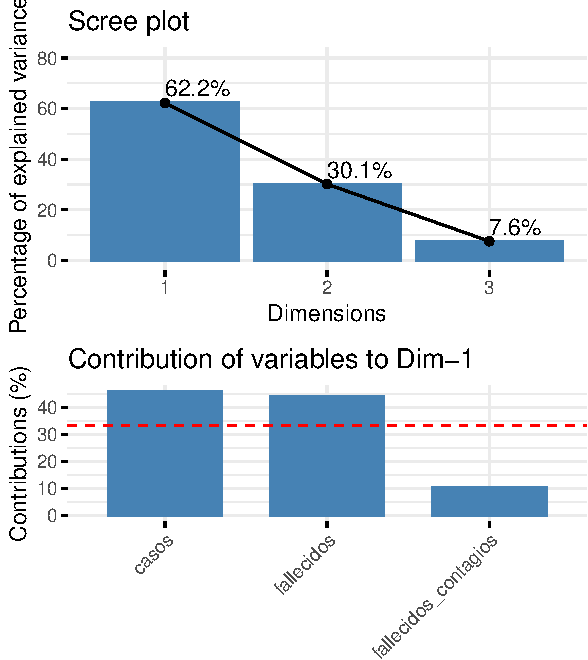
\includegraphics{Anexo_PCA_files/figure-latex/unnamed-chunk-1-1.pdf}

\hypertarget{crecimiento-econuxf3micoy-productivo}{%
\subsubsection{Crecimiento económicoy
productivo}\label{crecimiento-econuxf3micoy-productivo}}

Esta dimesión está compuesta por 2 variables. Las principales
estadísticas descriptivas son las siguientes:

\begin{table}
\centering\begingroup\fontsize{7}{9}\selectfont

\begin{tabular}{ll}
\toprule
Variable & N = 32\\
\midrule
Índice de diversidad económica & \\
\hspace{1em}Mean (SD) & 16.62 (5.88)\\
\hspace{1em}Median (IQR) & 14.46 (12.14, 20.64)\\
\hspace{1em}Range & 9.93, 34.44\\
Logaritmo de la intensidad lumínica promedio & \\
\addlinespace
\hspace{1em}Mean (SD) & -2.29 (2.45)\\
\hspace{1em}Median (IQR) & -1.57 (-2.77, -1.03)\\
\hspace{1em}Range & -7.24, 2.56\\
\bottomrule
\end{tabular}
\endgroup{}
\end{table}

Cada una de las variables fueron centradas y se realizó el análisis de
Componentes principales. Los siguientes gráficos muestran las
correlaciones de cada uno de las variables con los componentes
(dimensiones), resultado del análisis de ACP:

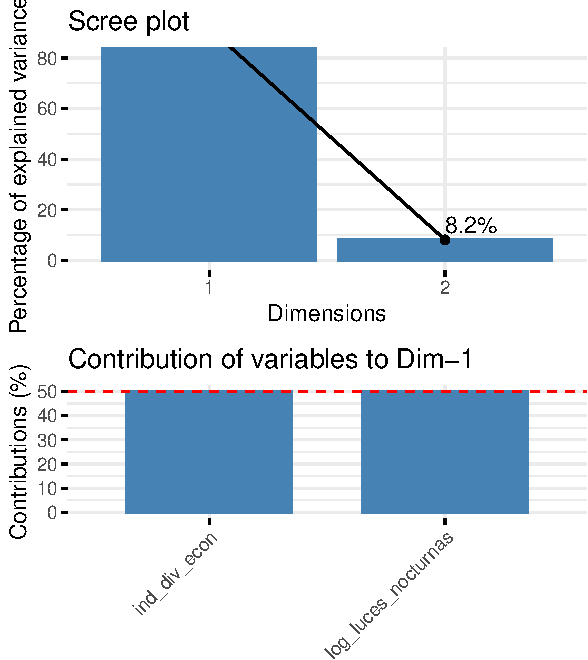
\includegraphics{Anexo_PCA_files/figure-latex/unnamed-chunk-1-2.pdf}

\hypertarget{acceso-a-servicio-de-agua-potable-y-saneamiento}{%
\subsubsection{Acceso a servicio de agua potable y
saneamiento}\label{acceso-a-servicio-de-agua-potable-y-saneamiento}}

Esta dimesión está compuesta por 12 variables. Las principales
estadísticas descriptivas son las siguientes:

\begin{table}
\centering\begingroup\fontsize{7}{9}\selectfont

\begin{tabular}{ll}
\toprule
Variable & N = 33\\
\midrule
Fuente de agua - aguatero & \\
\hspace{1em}Mean (SD) & 0.45 (0.78)\\
\hspace{1em}Median (IQR) & 0.06 (0.01, 0.37)\\
\hspace{1em}Range & 0.00, 2.65\\
Fuente de agua - acueducto público & \\
\addlinespace
\hspace{1em}Mean (SD) & 58.45 (26.05)\\
\hspace{1em}Median (IQR) & 65.79 (42.95, 76.47)\\
\hspace{1em}Range & 0.83, 98.92\\
Fuente de agua - acueducto comunal & \\
\hspace{1em}Mean (SD) & 10.72 (8.99)\\
\addlinespace
\hspace{1em}Median (IQR) & 8.57 (4.85, 13.82)\\
\hspace{1em}Range & 0.00, 34.48\\
Fuente de agua - pozo bomba & \\
\hspace{1em}Mean (SD) & 6.80 (9.48)\\
\hspace{1em}Median (IQR) & 2.69 (0.53, 9.91)\\
\addlinespace
\hspace{1em}Range & 0.03, 37.06\\
Fuente de agua - pozo no bomba & \\
\hspace{1em}Mean (SD) & 4.41 (6.47)\\
\hspace{1em}Median (IQR) & 2.63 (0.36, 4.87)\\
\hspace{1em}Range & 0.07, 30.23\\
\addlinespace
Fuente de agua - agua lluvia & \\
\hspace{1em}Mean (SD) & 7.79 (19.37)\\
\hspace{1em}Median (IQR) & 0.56 (0.22, 2.39)\\
\hspace{1em}Range & 0.00, 84.58\\
Fuente de agua - rio quebrada & \\
\addlinespace
\hspace{1em}Mean (SD) & 7.44 (10.62)\\
\hspace{1em}Median (IQR) & 5.23 (1.97, 7.86)\\
\hspace{1em}Range & 0.00, 59.63\\
Fuente de agua - agua botella o bolsa & \\
\hspace{1em}Mean (SD) & 2.89 (7.38)\\
\addlinespace
\hspace{1em}Median (IQR) & 0.73 (0.24, 2.24)\\
\hspace{1em}Range & 0.02, 41.13\\
Fuente de agua - pila pública & \\
\hspace{1em}Mean (SD) & 0.22 (0.38)\\
\hspace{1em}Median (IQR) & 0.05 (0.00, 0.17)\\
\addlinespace
\hspace{1em}Range & 0.00, 1.56\\
Fuente de agua - carrotanque & \\
\hspace{1em}Mean (SD) & 0.82 (2.23)\\
\hspace{1em}Median (IQR) & 0.02 (0.00, 0.42)\\
\hspace{1em}Range & 0.00, 10.35\\
\addlinespace
Saneamiento dentro de la vivienda & \\
\hspace{1em}Mean (SD) & 71.56 (22.76)\\
\hspace{1em}Median (IQR) & 70.73 (57.74, 92.69)\\
\hspace{1em}Range & 17.90, 98.74\\
Saneamiento fuera de la vivienda & \\
\addlinespace
\hspace{1em}Mean (SD) & 18.34 (12.47)\\
\hspace{1em}Median (IQR) & 18.20 (6.32, 28.93)\\
\hspace{1em}Range & 1.25, 39.79\\
\bottomrule
\end{tabular}
\endgroup{}
\end{table}

Cada una de las variables fueron centradas y se realizó el análisis de
Componentes principales. Los siguientes gráficos muestran las
correlaciones de cada uno de las variables con los componentes
(dimensiones), resultado del análisis de ACP:

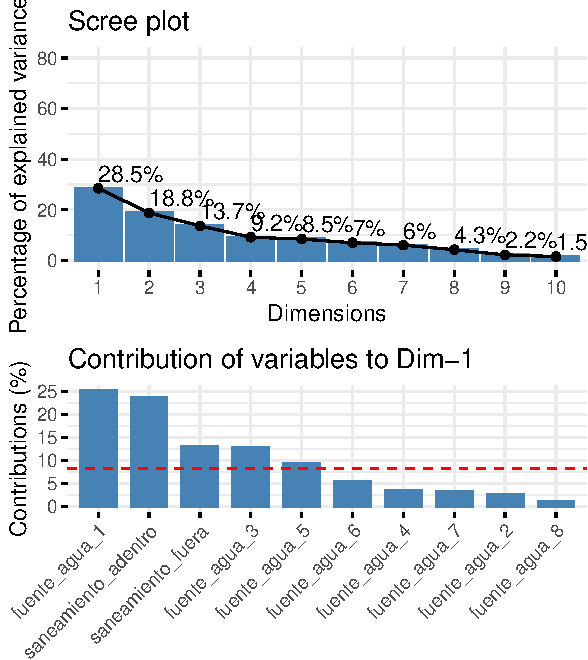
\includegraphics{Anexo_PCA_files/figure-latex/unnamed-chunk-1-3.pdf}

\hypertarget{caracteruxedsticas-de-las-viviendas}{%
\subsubsection{Características de las
Viviendas}\label{caracteruxedsticas-de-las-viviendas}}

Esta dimesión está compuesta por 16 variables. Las principales
estadísticas descriptivas son las siguientes:

\begin{table}
\centering\begingroup\fontsize{7}{9}\selectfont

\begin{tabular}{ll}
\toprule
Variable & N = 33\\
\midrule
Hacinamiento crítico (\%) & \\
\hspace{1em}Mean (SD) & 10.45 (6.70)\\
\hspace{1em}Median (IQR) & 8.60 (5.10, 14.20)\\
\hspace{1em}Range & 3.40, 31.10\\
Material de la pared - ladrillo & \\
\addlinespace
\hspace{1em}Mean (SD) & 74.40 (20.95)\\
\hspace{1em}Median (IQR) & 82.37 (63.20, 90.36)\\
\hspace{1em}Range & 18.65, 98.95\\
Material de la pared - bahareque no revo & \\
\hspace{1em}Mean (SD) & 2.54 (5.35)\\
\addlinespace
\hspace{1em}Median (IQR) & 0.40 (0.10, 3.57)\\
\hspace{1em}Range & 0.00, 29.44\\
Material de la pared - bahareque revo & \\
\hspace{1em}Mean (SD) & 2.72 (3.78)\\
\hspace{1em}Median (IQR) & 0.95 (0.12, 3.34)\\
\addlinespace
\hspace{1em}Range & 0.00, 13.83\\
Material de la pared - guadua & \\
\hspace{1em}Mean (SD) & 0.09 (0.11)\\
\hspace{1em}Median (IQR) & 0.05 (0.01, 0.12)\\
\hspace{1em}Range & 0.00, 0.46\\
\addlinespace
Material de la pared - latas deshechables & \\
\hspace{1em}Mean (SD) & 1.28 (3.26)\\
\hspace{1em}Median (IQR) & 0.12 (0.03, 0.49)\\
\hspace{1em}Range & 0.00, 17.29\\
Material de la pared - madera & \\
\addlinespace
\hspace{1em}Mean (SD) & 15.58 (17.79)\\
\hspace{1em}Median (IQR) & 7.34 (2.64, 22.60)\\
\hspace{1em}Range & 0.45, 64.95\\
Material de la pared - no hay & \\
\hspace{1em}Mean (SD) & 1.42 (2.14)\\
\addlinespace
\hspace{1em}Median (IQR) & 0.52 (0.18, 1.54)\\
\hspace{1em}Range & 0.06, 8.39\\
Material de la pared - prefabricado & \\
\hspace{1em}Mean (SD) & 0.49 (0.56)\\
\hspace{1em}Median (IQR) & 0.27 (0.13, 0.55)\\
\addlinespace
\hspace{1em}Range & 0.02, 2.63\\
Material de la pared - tapia & \\
\hspace{1em}Mean (SD) & 1.31 (2.70)\\
\hspace{1em}Median (IQR) & 0.18 (0.02, 0.52)\\
\hspace{1em}Range & 0.00, 11.61\\
\addlinespace
Material del piso - madera & \\
\hspace{1em}Mean (SD) & 0.91 (1.62)\\
\hspace{1em}Median (IQR) & 0.31 (0.14, 1.18)\\
\hspace{1em}Range & 0.00, 8.55\\
Material del piso - marmol & \\
\addlinespace
\hspace{1em}Mean (SD) & 0.23 (0.41)\\
\hspace{1em}Median (IQR) & 0.06 (0.02, 0.20)\\
\hspace{1em}Range & 0.00, 1.72\\
Material del piso - baldosa & \\
\hspace{1em}Mean (SD) & 46.67 (22.77)\\
\addlinespace
\hspace{1em}Median (IQR) & 47.61 (28.75, 68.01)\\
\hspace{1em}Range & 6.04, 80.80\\
Material del piso - madera burda & \\
\hspace{1em}Mean (SD) & 7.64 (12.69)\\
\hspace{1em}Median (IQR) & 2.19 (0.90, 5.08)\\
\addlinespace
\hspace{1em}Range & 0.16, 46.84\\
Material del piso - cemento & \\
\hspace{1em}Mean (SD) & 32.20 (12.86)\\
\hspace{1em}Median (IQR) & 33.19 (19.32, 41.93)\\
\hspace{1em}Range & 6.46, 57.16\\
\addlinespace
Material del piso - tierra & \\
\hspace{1em}Mean (SD) & 12.12 (15.39)\\
\hspace{1em}Median (IQR) & 5.06 (1.94, 17.21)\\
\hspace{1em}Range & 0.27, 66.37\\
\bottomrule
\end{tabular}
\endgroup{}
\end{table}

Cada una de las variables fueron centradas y se realizó el análisis de
Componentes principales. Los siguientes gráficos muestran las
correlaciones de cada uno de las variables con los componentes
(dimensiones), resultado del análisis de ACP:

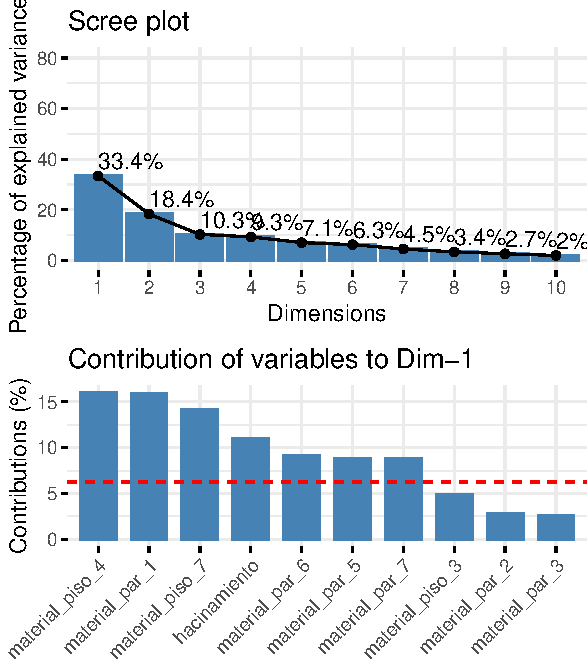
\includegraphics{Anexo_PCA_files/figure-latex/unnamed-chunk-1-4.pdf}

\hypertarget{desigualdad}{%
\subsubsection{Desigualdad}\label{desigualdad}}

Esta dimesión está compuesta por 1 variables. Las principales
estadísticas descriptivas son las siguientes:

\begin{table}
\centering\begingroup\fontsize{7}{9}\selectfont

\begin{tabular}{ll}
\toprule
Variable & N = 24\\
\midrule
Coeficiente de Gini & \\
\hspace{1em}Mean (SD) & 0.51 (0.03)\\
\hspace{1em}Median (IQR) & 0.51 (0.48, 0.52)\\
\hspace{1em}Range & 0.46, 0.56\\
\bottomrule
\end{tabular}
\endgroup{}
\end{table}

\hypertarget{pobreza}{%
\subsubsection{Pobreza}\label{pobreza}}

Esta dimesión está compuesta por 4 variables. Las principales
estadísticas descriptivas son las siguientes:

\begin{table}
\centering\begingroup\fontsize{7}{9}\selectfont

\begin{tabular}{ll}
\toprule
Variable & N = 33\\
\midrule
IPM (\%) & \\
\hspace{1em}Mean (SD) & 27.68 (17.27)\\
\hspace{1em}Median (IQR) & 26.10 (14.10, 33.40)\\
\hspace{1em}Range & 7.50, 75.60\\
nbietnia1 & \\
\addlinespace
\hspace{1em}Mean (SD) & 38.67 (22.08)\\
\hspace{1em}Median (IQR) & 36.74 (21.60, 53.67)\\
\hspace{1em}Range & 6.70, 91.12\\
nbietnia2 & \\
\hspace{1em}Mean (SD) & 17.50 (9.27)\\
\addlinespace
\hspace{1em}Median (IQR) & 16.48 (9.70, 23.32)\\
\hspace{1em}Range & 3.46, 41.99\\
NBI (\%) & \\
\hspace{1em}Mean (SD) & 24.20 (18.78)\\
\hspace{1em}Median (IQR) & 18.27 (10.67, 28.98)\\
\addlinespace
\hspace{1em}Range & 3.36, 68.89\\
\bottomrule
\end{tabular}
\endgroup{}
\end{table}

Cada una de las variables fueron centradas y se realizó el análisis de
Componentes principales. Los siguientes gráficos muestran las
correlaciones de cada uno de las variables con los componentes
(dimensiones), resultado del análisis de ACP:

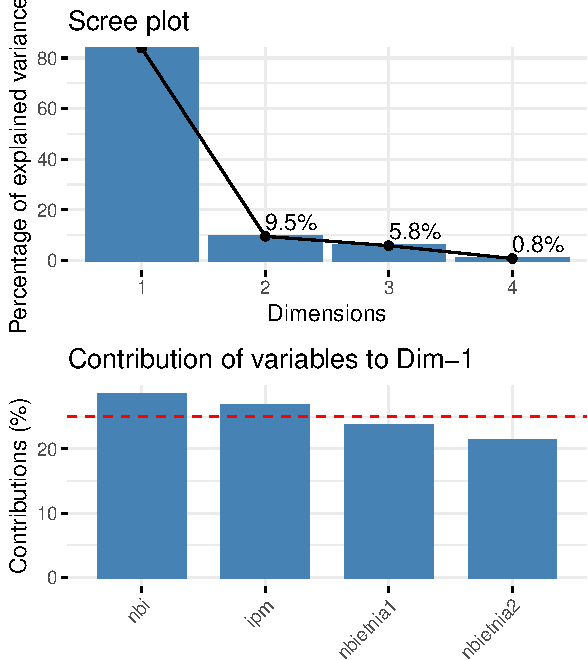
\includegraphics{Anexo_PCA_files/figure-latex/unnamed-chunk-1-5.pdf}

\hypertarget{cambio-climuxe1tico}{%
\subsubsection{Cambio Climático}\label{cambio-climuxe1tico}}

Esta dimesión está compuesta por 1 variables. Las principales
estadísticas descriptivas son las siguientes:

\begin{table}
\centering\begingroup\fontsize{7}{9}\selectfont

\begin{tabular}{ll}
\toprule
Variable & N = 33\\
\midrule
Área vulnerable al cambio climático & \\
\hspace{1em}Mean (SD) & 7.01 (20.04)\\
\hspace{1em}Median (IQR) & 0.21 (0.03, 3.05)\\
\hspace{1em}Range & 0.00, 98.56\\
\bottomrule
\end{tabular}
\endgroup{}
\end{table}

Cada una de las variables fueron centradas y se realizó el análisis de
Componentes principales. Los siguientes gráficos muestran las
correlaciones de cada uno de las variables con los componentes
(dimensiones), resultado del análisis de ACP:

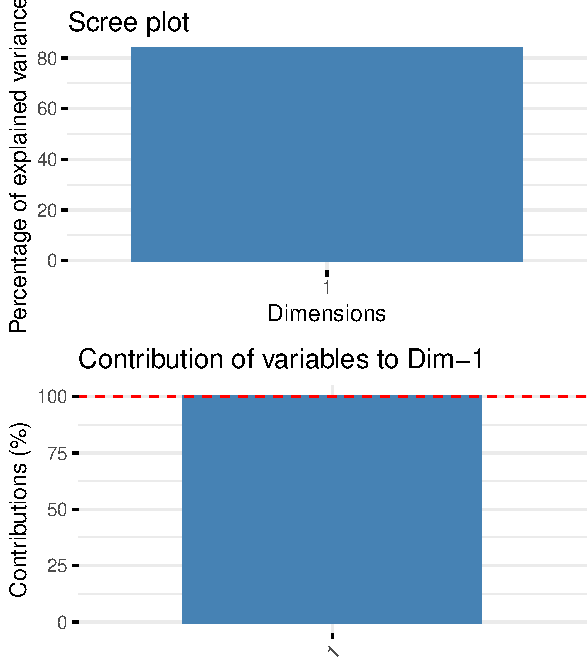
\includegraphics{Anexo_PCA_files/figure-latex/unnamed-chunk-1-6.pdf}

\hypertarget{estructura-demogruxe1fica}{%
\subsubsection{Estructura demográfica}\label{estructura-demogruxe1fica}}

Esta dimesión está compuesta por 4 variables. Las principales
estadísticas descriptivas son las siguientes:

\begin{table}
\centering\begingroup\fontsize{7}{9}\selectfont

\begin{tabular}{ll}
\toprule
Variable & N = 33\\
\midrule
poblacion\_etariagrupo1 & \\
\hspace{1em}Mean (SD) & 42.50 (5.10)\\
\hspace{1em}Median (IQR) & 43.87 (41.33, 45.09)\\
\hspace{1em}Range & 26.48, 50.80\\
poblacion\_etariagrupo2 & \\
\addlinespace
\hspace{1em}Mean (SD) & 23.16 (4.82)\\
\hspace{1em}Median (IQR) & 23.03 (19.78, 25.31)\\
\hspace{1em}Range & 16.17, 36.47\\
poblacion\_etariagrupo3 & \\
\hspace{1em}Mean (SD) & 24.59 (3.18)\\
\addlinespace
\hspace{1em}Median (IQR) & 24.05 (22.21, 26.25)\\
\hspace{1em}Range & 19.87, 33.11\\
poblacion\_etariagrupo4 & \\
\hspace{1em}Mean (SD) & 9.75 (3.24)\\
\hspace{1em}Median (IQR) & 9.98 (7.56, 11.73)\\
\addlinespace
\hspace{1em}Range & 3.94, 16.03\\
\bottomrule
\end{tabular}
\endgroup{}
\end{table}

Cada una de las variables fueron centradas y se realizó el análisis de
Componentes principales. Los siguientes gráficos muestran las
correlaciones de cada uno de las variables con los componentes
(dimensiones), resultado del análisis de ACP:

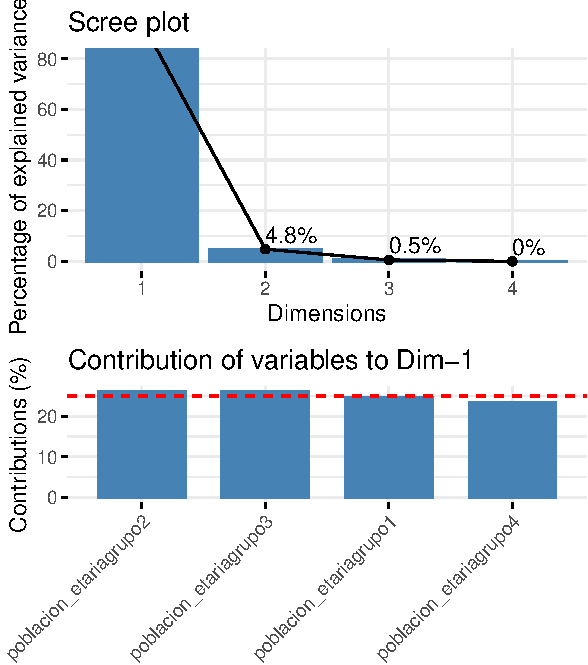
\includegraphics{Anexo_PCA_files/figure-latex/unnamed-chunk-1-7.pdf}

\hypertarget{resultados}{%
\subsection{Resultados}\label{resultados}}

\hypertarget{infancia-y-niuxf1ez}{%
\subsubsection{Infancia y Niñez}\label{infancia-y-niuxf1ez}}

Esta dimesión está compuesta por 17 variables. Las principales
estadísticas descriptivas son las siguientes:

\begin{table}
\centering\begingroup\fontsize{7}{9}\selectfont

\begin{tabular}{ll}
\toprule
Variable & N = 33\\
\midrule
Asistencia escolar de menores de 5 años por quintil de ingreso (\%) - quintil 1 & \\
\hspace{1em}Mean (SD) & 21.32 (12.81)\\
\hspace{1em}Median (IQR) & 18.91 (13.51, 27.53)\\
\hspace{1em}Range & 1.90, 48.68\\
Asistencia escolar de menores de 5 años por quintil de ingreso (\%) - quintil 2 & \\
\addlinespace
\hspace{1em}Mean (SD) & 21.50 (12.29)\\
\hspace{1em}Median (IQR) & 23.67 (9.44, 30.78)\\
\hspace{1em}Range & 2.47, 47.37\\
Asistencia escolar de menores de 5 años por quintil de ingreso (\%) - quintil 3 & \\
\hspace{1em}Mean (SD) & 20.91 (12.92)\\
\addlinespace
\hspace{1em}Median (IQR) & 21.95 (11.21, 26.20)\\
\hspace{1em}Range & 0.00, 53.91\\
Asistencia escolar de menores de 5 años por quintil de ingreso (\%) - quintil 4 & \\
\hspace{1em}Mean (SD) & 20.89 (12.21)\\
\hspace{1em}Median (IQR) & 20.64 (12.29, 28.30)\\
\addlinespace
\hspace{1em}Range & 3.10, 55.37\\
Asistencia escolar de menores de 5 años por quintil de ingreso (\%) - quintil 5 & \\
\hspace{1em}Mean (SD) & 22.74 (11.92)\\
\hspace{1em}Median (IQR) & 22.32 (14.64, 31.05)\\
\hspace{1em}Range & 3.33, 44.24\\
\addlinespace
Asistencia escolar de menores de 5 años (\%) & \\
\hspace{1em}Mean (SD) & 19.48 (10.74)\\
\hspace{1em}Median (IQR) & 18.48 (11.16, 27.44)\\
\hspace{1em}Range & 2.11, 43.26\\
Asistencia escolar a educación primaria por quintil de ingreso (\%) - quintil 1 & \\
\addlinespace
\hspace{1em}Mean (SD) & 51.15 (16.26)\\
\hspace{1em}Median (IQR) & 48.41 (42.27, 54.28)\\
\hspace{1em}Range & 27.53, 100.00\\
Asistencia escolar a educación primaria por quintil de ingreso (\%) - quintil 2 & \\
\hspace{1em}Mean (SD) & 47.32 (16.91)\\
\addlinespace
\hspace{1em}Median (IQR) & 46.02 (37.60, 54.27)\\
\hspace{1em}Range & 10.00, 85.98\\
Asistencia escolar a educación primaria por quintil de ingreso (\%) - quintil 3 & \\
\hspace{1em}Mean (SD) & 45.75 (17.23)\\
\hspace{1em}Median (IQR) & 42.58 (37.32, 53.36)\\
\addlinespace
\hspace{1em}Range & 12.23, 100.00\\
Asistencia escolar a educación primaria por quintil de ingreso (\%) - quintil 4 & \\
\hspace{1em}Mean (SD) & 56.01 (10.97)\\
\hspace{1em}Median (IQR) & 55.44 (49.64, 63.98)\\
\hspace{1em}Range & 22.45, 75.68\\
\addlinespace
Asistencia escolar a educación primaria por quintil de ingreso (\%) - quintil 5 & \\
\hspace{1em}Mean (SD) & 74.52 (12.42)\\
\hspace{1em}Median (IQR) & 75.48 (65.24, 84.50)\\
\hspace{1em}Range & 50.13, 99.25\\
Asistencia escolar a educación primaria (\%) & \\
\addlinespace
\hspace{1em}Mean (SD) & 51.03 (3.91)\\
\hspace{1em}Median (IQR) & 51.13 (49.59, 52.29)\\
\hspace{1em}Range & 37.22, 59.94\\
Tasa de mortalidad infantil en menores de 5 años en los últimos 10 años & \\
\hspace{1em}Mean (SD) & 21.18 (11.63)\\
\addlinespace
\hspace{1em}Median (IQR) & 17.00 (15.00, 23.00)\\
\hspace{1em}Range & 6.00, 60.00\\
Tasa de mortalidad infantil en los últimos 10 años & \\
\hspace{1em}Mean (SD) & 17.67 (9.32)\\
\hspace{1em}Median (IQR) & 15.00 (12.00, 18.00)\\
\addlinespace
\hspace{1em}Range & 4.00, 46.00\\
Tasa de mortalidad infantil & \\
\hspace{1em}Mean (SD) & 11.31 (4.17)\\
\hspace{1em}Median (IQR) & 10.01 (9.08, 12.51)\\
\hspace{1em}Range & 6.51, 24.10\\
\addlinespace
Nacidos vivos en los últimos 5 años (\%) & \\
\hspace{1em}Mean (SD) & 93.18 (13.13)\\
\hspace{1em}Median (IQR) & 98.00 (94.20, 99.50)\\
\hspace{1em}Range & 36.60, 100.00\\
Tamaño de clase en primaria & \\
\addlinespace
\hspace{1em}Mean (SD) & 19.06 (4.24)\\
\hspace{1em}Median (IQR) & 19.91 (15.13, 22.13)\\
\hspace{1em}Range & 10.80, 27.09\\
\bottomrule
\end{tabular}
\endgroup{}
\end{table}

Cada una de las variables fueron centradas y se realizó el análisis de
Componentes principales. Los siguientes gráficos muestran las
correlaciones de cada uno de las variables con los componentes
(dimensiones), resultado del análisis de ACP:

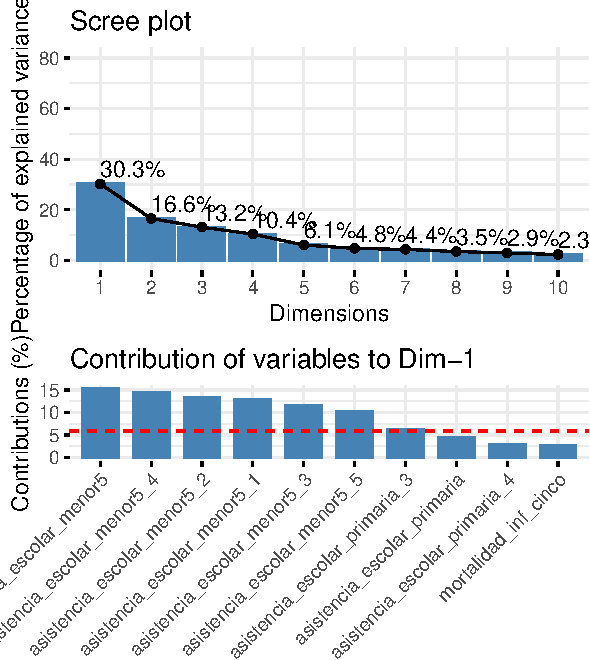
\includegraphics{Anexo_PCA_files/figure-latex/unnamed-chunk-1-8.pdf}

\hypertarget{juventud}{%
\subsubsection{Juventud}\label{juventud}}

Esta dimesión está compuesta por 20 variables. Las principales
estadísticas descriptivas son las siguientes:

\begin{table}
\centering\begingroup\fontsize{7}{9}\selectfont

\begin{tabular}{ll}
\toprule
Variable & N = 30\\
\midrule
Asistencia escolar de 13 a 17 años por quintil de ingreso (\%) - quintil 1 & \\
\hspace{1em}Mean (SD) & 64.72 (13.88)\\
\hspace{1em}Median (IQR) & 64.26 (53.72, 74.53)\\
\hspace{1em}Range & 41.09, 93.47\\
Asistencia escolar de 13 a 17 años por quintil de ingreso (\%) - quintil 2 & \\
\addlinespace
\hspace{1em}Mean (SD) & 73.05 (12.11)\\
\hspace{1em}Median (IQR) & 71.15 (64.05, 80.96)\\
\hspace{1em}Range & 56.00, 100.00\\
Asistencia escolar de 13 a 17 años por quintil de ingreso (\%) - quintil 3 & \\
\hspace{1em}Mean (SD) & 77.55 (16.24)\\
\addlinespace
\hspace{1em}Median (IQR) & 74.62 (66.16, 91.84)\\
\hspace{1em}Range & 35.75, 100.00\\
Asistencia escolar de 13 a 17 años por quintil de ingreso (\%) - quintil 4 & \\
\hspace{1em}Mean (SD) & 79.74 (11.75)\\
\hspace{1em}Median (IQR) & 80.38 (72.52, 87.85)\\
\addlinespace
\hspace{1em}Range & 56.15, 99.85\\
Asistencia escolar de 13 a 17 años por quintil de ingreso (\%) - quintil 5 & \\
\hspace{1em}Mean (SD) & 91.03 (10.04)\\
\hspace{1em}Median (IQR) & 94.30 (84.61, 100.00)\\
\hspace{1em}Range & 64.08, 100.00\\
\addlinespace
Asistencia escolar de 13 a 17 años (\%) & \\
\hspace{1em}Mean (SD) & 68.16 (7.47)\\
\hspace{1em}Median (IQR) & 68.42 (64.60, 71.14)\\
\hspace{1em}Range & 41.96, 83.77\\
Diferencias en la terminación de educación secundaria entre indígenas y no indígenas & \\
\addlinespace
\hspace{1em}Mean (SD) & -21.49 (21.81)\\
\hspace{1em}Median (IQR) & -22.72 (-38.16, -14.07)\\
\hspace{1em}Range & -49.03, 48.40\\
Edad promedio del primer matrimonio & \\
\hspace{1em}Mean (SD) & 20.53 (1.30)\\
\addlinespace
\hspace{1em}Median (IQR) & 20.55 (19.58, 21.45)\\
\hspace{1em}Range & 17.60, 22.90\\
Edad promedio del primer encuentro sexual de mujeres entre 15 y 49 años & \\
\hspace{1em}Mean (SD) & 17.22 (0.83)\\
\hspace{1em}Median (IQR) & 17.35 (16.62, 17.85)\\
\addlinespace
\hspace{1em}Range & 14.90, 18.40\\
Jóvenes de 18 a 28 años han asistido a una institución de educación superior (\%) & \\
\hspace{1em}Mean (SD) & 22.51 (7.86)\\
\hspace{1em}Median (IQR) & 22.71 (17.64, 27.04)\\
\hspace{1em}Range & 7.51, 43.16\\
\addlinespace
Tasa de fecundidad de mujeres jóvenes & \\
\hspace{1em}Mean (SD) & 63.69 (17.59)\\
\hspace{1em}Median (IQR) & 58.72 (49.90, 78.19)\\
\hspace{1em}Range & 34.44, 96.19\\
Tasa de fertilidad últimos tres años en mujeres de 15 a 49 años & \\
\addlinespace
\hspace{1em}Mean (SD) & 2.29 (0.70)\\
\hspace{1em}Median (IQR) & 2.20 (1.80, 2.55)\\
\hspace{1em}Range & 1.30, 4.60\\
Mujeres con educación secundaria o superior (\%) & \\
\hspace{1em}Mean (SD) & 78.21 (7.54)\\
\addlinespace
\hspace{1em}Median (IQR) & 80.00 (74.77, 81.80)\\
\hspace{1em}Range & 56.30, 91.80\\
Rezago escolar de 13 a 17 años por quintil de ingreso (\%) - quintil 1 & \\
\hspace{1em}Mean (SD) & 40.25 (17.57)\\
\hspace{1em}Median (IQR) & 39.92 (32.10, 51.50)\\
\addlinespace
\hspace{1em}Range & 0.00, 69.84\\
Rezago escolar de 13 a 17 años por quintil de ingreso (\%) - quintil 2 & \\
\hspace{1em}Mean (SD) & 42.20 (20.18)\\
\hspace{1em}Median (IQR) & 41.23 (30.50, 51.25)\\
\hspace{1em}Range & 0.00, 99.28\\
\addlinespace
Rezago escolar de 13 a 17 años por quintil de ingreso (\%) - quintil 3 & \\
\hspace{1em}Mean (SD) & 47.41 (28.00)\\
\hspace{1em}Median (IQR) & 42.96 (28.78, 63.43)\\
\hspace{1em}Range & 0.00, \vphantom{1} 100.00\\
Rezago escolar de 13 a 17 años por quintil de ingreso (\%) - quintil 4 & \\
\addlinespace
\hspace{1em}Mean (SD) & 41.37 (20.33)\\
\hspace{1em}Median (IQR) & 38.96 (30.83, 54.08)\\
\hspace{1em}Range & 0.00, 82.75\\
Rezago escolar de 13 a 17 años por quintil de ingreso (\%) - quintil 5 & \\
\hspace{1em}Mean (SD) & 66.37 (26.08)\\
\addlinespace
\hspace{1em}Median (IQR) & 63.70 (50.72, 84.44)\\
\hspace{1em}Range & 0.00, 100.00\\
Rezago escolar de 13 a 17 años (\%) & \\
\hspace{1em}Mean (SD) & 44.51 (5.61)\\
\hspace{1em}Median (IQR) & 44.34 (41.99, 48.00)\\
\addlinespace
\hspace{1em}Range & 29.02, 55.51\\
Tamaño de clase en secundaria y media & \\
\hspace{1em}Mean (SD) & 19.64 (2.48)\\
\hspace{1em}Median (IQR) & 20.20 (18.22, 21.66)\\
\hspace{1em}Range & 14.79, 23.37\\
\bottomrule
\end{tabular}
\endgroup{}
\end{table}

Cada una de las variables fueron centradas y se realizó el análisis de
Componentes principales. Los siguientes gráficos muestran las
correlaciones de cada uno de las variables con los componentes
(dimensiones), resultado del análisis de ACP:

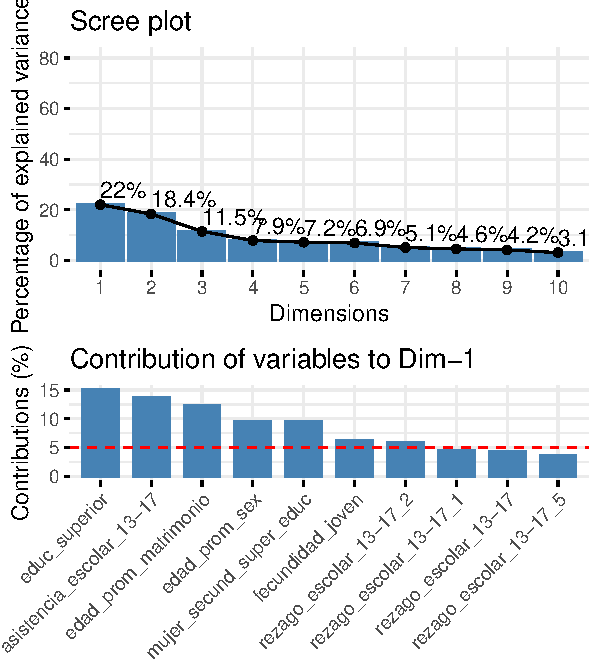
\includegraphics{Anexo_PCA_files/figure-latex/unnamed-chunk-1-9.pdf}

\hypertarget{adultez}{%
\subsubsection{Adultez}\label{adultez}}

Esta dimesión está compuesta por 16 variables. Las principales
estadísticas descriptivas son las siguientes:

\begin{table}
\centering\begingroup\fontsize{7}{9}\selectfont

\begin{tabular}{ll}
\toprule
Variable & N = 33\\
\midrule
homicidiosedad6 & \\
\hspace{1em}Mean (SD) & 0.19 (0.24)\\
\hspace{1em}Median (IQR) & 0.16 (0.00, 0.28)\\
\hspace{1em}Range & 0.00, 1.11\\
homicidiosedad7 & \\
\addlinespace
\hspace{1em}Mean (SD) & 18.25 (11.47)\\
\hspace{1em}Median (IQR) & 15.64 (10.43, 24.62)\\
\hspace{1em}Range & 4.43, 54.95\\
homicidiosedad8 & \\
\hspace{1em}Mean (SD) & 3.91 (2.09)\\
\addlinespace
\hspace{1em}Median (IQR) & 3.43 (2.61, 4.75)\\
\hspace{1em}Range & 0.00, 9.47\\
homicidiosedad9 & \\
\hspace{1em}Mean (SD) & 0.52 (0.35)\\
\hspace{1em}Median (IQR) & 0.56 (0.33, 0.73)\\
\addlinespace
\hspace{1em}Range & 0.00, 1.19\\
homicidiosgen1 & \\
\hspace{1em}Mean (SD) & 21.21 (12.20)\\
\hspace{1em}Median (IQR) & 17.79 (13.38, 28.39)\\
\hspace{1em}Range & 4.47, 58.09\\
\addlinespace
homicidiosgen2 & \\
\hspace{1em}Mean (SD) & 1.75 (1.07)\\
\hspace{1em}Median (IQR) & 1.43 (0.93, 2.30)\\
\hspace{1em}Range & 0.00, 4.22\\
Agresiones (homicidios) & \\
\addlinespace
\hspace{1em}Mean (SD) & 22.96 (12.99)\\
\hspace{1em}Median (IQR) & 19.17 (14.33, 30.30)\\
\hspace{1em}Range & 4.47, 59.66\\
suicidios\_15\_64edad7 & \\
\hspace{1em}Mean (SD) & 4.17 \vphantom{1} (4.19)\\
\addlinespace
\hspace{1em}Median (IQR) & 3.09 (2.31, \vphantom{1} 4.39)\\
\hspace{1em}Range & 0.83, \vphantom{1} 20.13\\
suicidios\_15\_64edad8 & \\
\hspace{1em}Mean (SD) & 1.21 \vphantom{1} (0.83)\\
\hspace{1em}Median (IQR) & 1.19 (0.73, \vphantom{1} 1.44)\\
\addlinespace
\hspace{1em}Range & 0.00, \vphantom{1} 4.71\\
suicidiosedad6 & \\
\hspace{1em}Mean (SD) & 0.33 (0.42)\\
\hspace{1em}Median (IQR) & 0.19 (0.11, 0.40)\\
\hspace{1em}Range & 0.00, 2.24\\
\addlinespace
suicidiosedad7 & \\
\hspace{1em}Mean (SD) & 4.17 (4.19)\\
\hspace{1em}Median (IQR) & 3.09 (2.31, 4.39)\\
\hspace{1em}Range & 0.83, 20.13\\
suicidiosedad8 & \\
\addlinespace
\hspace{1em}Mean (SD) & 1.21 (0.83)\\
\hspace{1em}Median (IQR) & 1.19 (0.73, 1.44)\\
\hspace{1em}Range & 0.00, 4.71\\
suicidiosedad9 & \\
\hspace{1em}Mean (SD) & 0.59 (0.42)\\
\addlinespace
\hspace{1em}Median (IQR) & 0.61 (0.28, 0.80)\\
\hspace{1em}Range & 0.00, 1.62\\
suicidiosgen1 & \\
\hspace{1em}Mean (SD) & 4.84 (2.87)\\
\hspace{1em}Median (IQR) & 4.55 (3.21, 5.57)\\
\addlinespace
\hspace{1em}Range & 1.66, 17.72\\
suicidiosgen2 & \\
\hspace{1em}Mean (SD) & 1.46 (2.30)\\
\hspace{1em}Median (IQR) & 0.96 (0.66, 1.57)\\
\hspace{1em}Range & 0.00, 13.42\\
\addlinespace
Fallecidos por lesiones autoinfligidas intencionalmente (suicidios) & \\
\hspace{1em}Mean (SD) & 6.30 (4.42)\\
\hspace{1em}Median (IQR) & 5.76 (4.22, 6.51)\\
\hspace{1em}Range & 1.76, 22.37\\
\bottomrule
\end{tabular}
\endgroup{}
\end{table}

Cada una de las variables fueron centradas y se realizó el análisis de
Componentes principales. Los siguientes gráficos muestran las
correlaciones de cada uno de las variables con los componentes
(dimensiones), resultado del análisis de ACP:

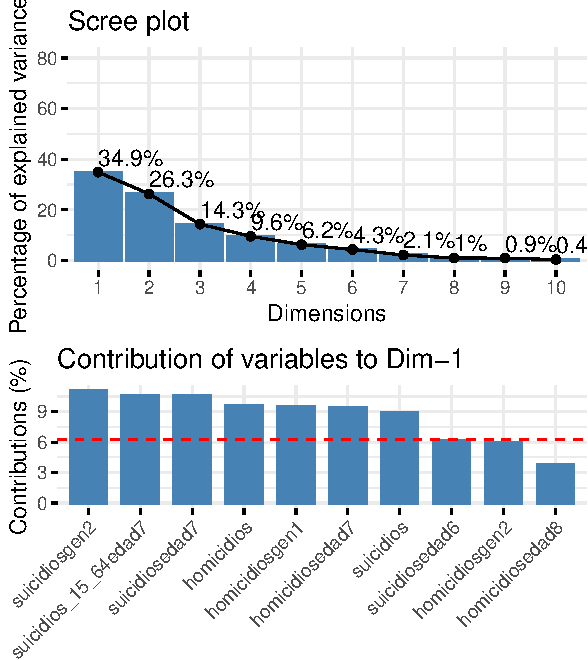
\includegraphics{Anexo_PCA_files/figure-latex/unnamed-chunk-1-10.pdf}

\hypertarget{vejez}{%
\subsubsection{Vejez}\label{vejez}}

Esta dimesión está compuesta por 6 variables. Las principales
estadísticas descriptivas son las siguientes:

\begin{table}
\centering\begingroup\fontsize{7}{9}\selectfont

\begin{tabular}{ll}
\toprule
Variable & N = 33\\
\midrule
defunciones\_entcausa1 & \\
\hspace{1em}Mean (SD) & 78.39 (32.66)\\
\hspace{1em}Median (IQR) & 77.95 (58.13, 100.96)\\
\hspace{1em}Range & 22.13, 152.85\\
defunciones\_entcausa2 & \\
\addlinespace
\hspace{1em}Mean (SD) & 139.31 (52.88)\\
\hspace{1em}Median (IQR) & 152.82 (108.04, 168.55)\\
\hspace{1em}Range & 38.02, 240.52\\
defunciones\_entcausa3 & \\
\hspace{1em}Mean (SD) & 56.60 (16.75)\\
\addlinespace
\hspace{1em}Median (IQR) & 56.04 (45.42, 67.10)\\
\hspace{1em}Range & 29.21, 92.63\\
defunciones\_entcausa4 & \\
\hspace{1em}Mean (SD) & 26.25 (12.17)\\
\hspace{1em}Median (IQR) & 25.37 (20.77, 31.83)\\
\addlinespace
\hspace{1em}Range & 4.47, 59.24\\
defunciones\_entcausa5 & \\
\hspace{1em}Mean (SD) & 18.62 (6.34)\\
\hspace{1em}Median (IQR) & 19.35 (13.94, 23.07)\\
\hspace{1em}Range & 2.24, 28.26\\
\addlinespace
Número de defunciones prematuras & \\
\hspace{1em}Mean (SD) & 187.70 (177.76)\\
\hspace{1em}Median (IQR) & 144.00 (48.00, 280.00)\\
\hspace{1em}Range & 5.00, 646.00\\
\bottomrule
\end{tabular}
\endgroup{}
\end{table}

Cada una de las variables fueron centradas y se realizó el análisis de
Componentes principales. Los siguientes gráficos muestran las
correlaciones de cada uno de las variables con los componentes
(dimensiones), resultado del análisis de ACP:

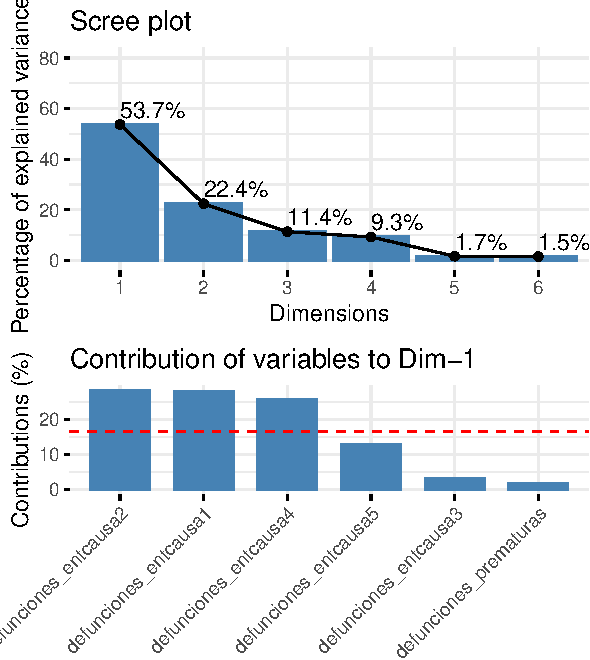
\includegraphics{Anexo_PCA_files/figure-latex/unnamed-chunk-1-11.pdf}